


\tikzset{every picture/.style={line width=0.75pt}} %set default line width to 0.75pt        

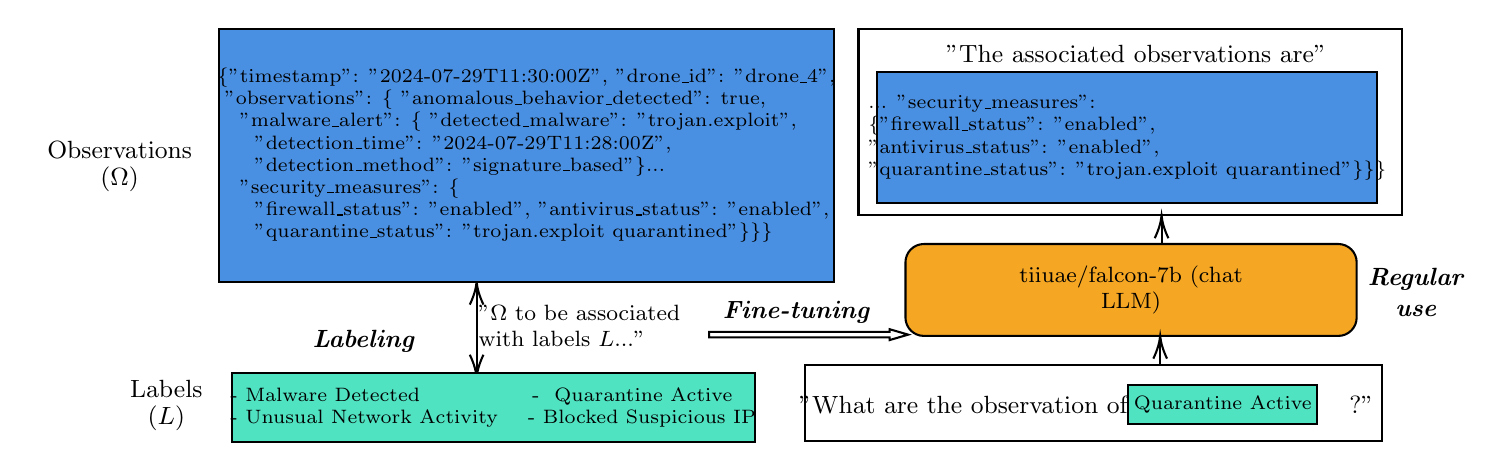
\begin{tikzpicture}[x=0.75pt,y=0.75pt,yscale=-1,xscale=1]
%uncomment if require: \path (0,1662); %set diagram left start at 0, and has height of 1662

%Rounded Rect [id:dp17386115134623514] 
\draw  [fill={rgb, 255:red, 245; green, 166; blue, 35 }  ,fill opacity=1 ] (424.61,402.58) .. controls (424.61,397.69) and (428.57,393.73) .. (433.46,393.73) -- (633.15,393.73) .. controls (638.04,393.73) and (642,397.69) .. (642,402.58) -- (642,429.15) .. controls (642,434.04) and (638.04,438) .. (633.15,438) -- (433.46,438) .. controls (428.57,438) and (424.61,434.04) .. (424.61,429.15) -- cycle ;
%Straight Lines [id:da8877910798706699] 
\draw    (547.33,451.83) -- (547.33,440) ;
\draw [shift={(547.33,438)}, rotate = 90] [color={rgb, 255:red, 0; green, 0; blue, 0 }  ][line width=0.75]    (10.93,-3.29) .. controls (6.95,-1.4) and (3.31,-0.3) .. (0,0) .. controls (3.31,0.3) and (6.95,1.4) .. (10.93,3.29)   ;
%Shape: Rectangle [id:dp44726237549140535] 
\draw   (376,452.18) -- (654,452.18) -- (654,488.66) -- (376,488.66) -- cycle ;
%Shape: Rectangle [id:dp2820683536345354] 
\draw   (402,290.27) -- (664,290.27) -- (664,379.64) -- (402,379.64) -- cycle ;
%Right Arrow [id:dp4162270206865013] 
\draw   (330,436.09) -- (417,436.09) -- (417,434.78) -- (425.91,437.39) -- (417,440) -- (417,438.7) -- (330,438.7) -- cycle ;
%Straight Lines [id:da8267677953106705] 
\draw    (548,393.83) -- (548,382) ;
\draw [shift={(548,380)}, rotate = 90] [color={rgb, 255:red, 0; green, 0; blue, 0 }  ][line width=0.75]    (10.93,-3.29) .. controls (6.95,-1.4) and (3.31,-0.3) .. (0,0) .. controls (3.31,0.3) and (6.95,1.4) .. (10.93,3.29)   ;
%Straight Lines [id:da6319519397458309] 
\draw    (218,456) -- (218,414) ;
\draw [shift={(218,412)}, rotate = 90] [color={rgb, 255:red, 0; green, 0; blue, 0 }  ][line width=0.75]    (10.93,-3.29) .. controls (6.95,-1.4) and (3.31,-0.3) .. (0,0) .. controls (3.31,0.3) and (6.95,1.4) .. (10.93,3.29)   ;
\draw [shift={(218,458)}, rotate = 270] [color={rgb, 255:red, 0; green, 0; blue, 0 }  ][line width=0.75]    (10.93,-3.29) .. controls (6.95,-1.4) and (3.31,-0.3) .. (0,0) .. controls (3.31,0.3) and (6.95,1.4) .. (10.93,3.29)   ;


% Text Node
\draw (68.5,471.5) node  [font=\footnotesize] [align=left] {\begin{minipage}[lt]{35.92pt}\setlength\topsep{0pt}
\begin{center}
{\small Labels ($\displaystyle L$)}
\end{center}

\end{minipage}};
% Text Node
\draw (372.5,426.5) node  [font=\small] [align=left] {\textit{\textbf{Fine-tuning}}};
% Text Node
\draw  [fill={rgb, 255:red, 74; green, 144; blue, 226 }  ,fill opacity=1 ]  (411,311) -- (652,311) -- (652,374) -- (411,374) -- cycle  ;
\draw (531.5,342.5) node  [font=\scriptsize] [align=left] {... "security\_measures":\\\{"firewall\_status": "enabled",\\"antivirus\_status": "enabled",\\"quarantine\_status": "trojan.exploit quarantined"\}\}\}};
% Text Node
\draw  [fill={rgb, 255:red, 80; green, 227; blue, 194 }  ,fill opacity=1 ]  (532,461.66) -- (623,461.66) -- (623,480.66) -- (532,480.66) -- cycle  ;
\draw (577.5,471.16) node  [font=\scriptsize] [align=left] {Quarantine Active};
% Text Node
\draw (536,302.25) node  [font=\footnotesize] [align=left] {{\small "The associated observations are"}};
% Text Node
\draw (671,417) node  [font=\small] [align=left] {\begin{minipage}[lt]{36.9pt}\setlength\topsep{0pt}
\begin{center}
\textit{\textbf{Regular}}\\\textit{\textbf{use}}
\end{center}

\end{minipage}};
% Text Node
\draw (512,471.16) node  [font=\footnotesize] [align=left] {{\small "What are the observation of \ \ \ \ \ \ \ \ \ \ \ \ \ \ \ \ \ \ \ \ \ \ \ \ \ ?"}};
% Text Node
\draw (46,356.32) node  [font=\footnotesize] [align=left] {\begin{minipage}[lt]{59.79pt}\setlength\topsep{0pt}
\begin{center}
{\small Observations ($\displaystyle \Omega $)}
\end{center}

\end{minipage}};
% Text Node
\draw (164,440.5) node  [font=\small] [align=left] {\textit{\textbf{Labeling}}};
% Text Node
\draw (267.5,433) node  [font=\footnotesize] [align=left] {{\footnotesize "$\displaystyle \Omega $ to be associated}\\{\footnotesize with labels $\displaystyle L$..."}};
% Text Node
\draw (533.3,415.86) node  [font=\footnotesize] [align=left] {\begin{minipage}[lt]{99.33pt}\setlength\topsep{0pt}
\begin{center}
tiiuae/falcon-7b (chat LLM)
\end{center}

\end{minipage}};
% Text Node
\draw  [fill={rgb, 255:red, 80; green, 227; blue, 194 }  ,fill opacity=1 ]  (100,456) -- (352,456) -- (352,489) -- (100,489) -- cycle  ;
\draw (226,472.5) node  [font=\scriptsize] [align=left] {\mbox{-} Malware Detected \ \ \ \ \ \ \ \ \ \ \ \ \ \ - \ Quarantine Active\\\mbox{-} Unusual Network Activity \ \ \ - Blocked Suspicious IP};
% Text Node
\draw  [fill={rgb, 255:red, 74; green, 144; blue, 226 }  ,fill opacity=1 ]  (94,290) -- (390,290) -- (390,412) -- (94,412) -- cycle  ;
\draw (242,351) node  [font=\scriptsize] [align=left] {\{"timestamp": "2024-07-29T11:30:00Z", "drone\_id": "drone\_4",\\ \ "observations": \{ "anomalous\_behavior\_detected": true,\\ \ \ \ "malware\_alert": \{ "detected\_malware": "trojan.exploit",\\ \ \ \ \ \ "detection\_time": "2024-07-29T11:28:00Z",\\ \ \ \ \ \ "detection\_method": "signature\_based"\}...\\ \ \ \ "security\_measures": \{\\ \ \ \ \ \ "firewall\_status": "enabled", "antivirus\_status": "enabled",\\ \ \ \ \ \ "quarantine\_status": "trojan.exploit quarantined"\}\}\}};


\end{tikzpicture}